%! Author = Saeid Yazdani
%! Date = 9/6/2024

\clearpage
\section{Messaging Protocol}
\label{sec:msg-protocol}

The communication between operators  (GUI application, \acs{ATE}, etc.)
and the MCU inside the \acs{HVS} utilizes a simple dynamically-sized
byte protocol for data exchange as shown in \autoref{fig:protocol-frame}.

The start and end of each message are marked by two consecutive bytes, making
up a total of four bytes for framing.
The payload varies in size and the participants in the protocol should
know the expected size of each message based on the command byte of the
message.
That is, the minimum message size is \emph{6}, and only one data byte
needs to be exchanged between the caller and the callee.

\begin{figure}[h]
    \centering
    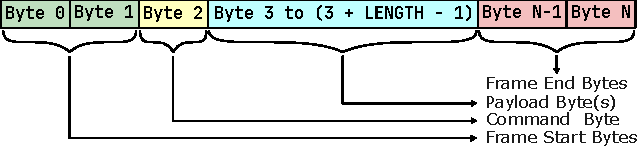
\includegraphics[width=0.8\textwidth]
    {figures/software/protocol-frame}
    \caption[Messaging Protocol Frame Structure]{
        The frame structure of messaging protocol for communicating with
        the \ac{HVS} system.
        A Frame size of $N$ bytes can be identified by two start bytes
        and two end (stop) bytes. The caller and callee must know the
        length of the payload beforehand based on the command byte.
    }
    \label{fig:protocol-frame}
\end{figure}


The communication operates at two distinct baud rates:

\begin{itemize}[topsep=8pt,itemsep=4pt,partopsep=4pt, parsep=4pt]
    \item \SI{115.2}{\kbd} for standard commands (set range, mode, value, etc.)
    \item \SI{512}{\kbd} for burst operations involving waveform or data-points
    transfers.
\end{itemize}

The communication is designed to be quasi-sequential.
That is, when a command is sent to the \acs{HVS} and a reply is expected,
the caller may issue a new message before receiving a reply for the
previously requested operation, but needs to keep track of the replies that are
sent back by the \acs{HVS} system.
For most of the commands, this is trivial since the reply will contain the
same command identifier and, in case of read and write, the address of which the
caller has made a request.

This is facilitated by the firmware in the MCU where for most of the commands it
uses a queue to service the requests.
For safety reasons, a few commands that will invalidate the queue and will
trigger an immediate reaction are provisioned, such as \emph{RESET\_FPGA}
where the output will be immediately stopped and all the registers of the
FPGA will be updated with their reset values.

Since the GUI software and MCU firmware are written in \emph{C++} and \emph{C},
they share a common header file which contains constants and masks for
generating and parsing the protocol as shown in
\autoref{lst:mcu-protocol-header}.
\newpage
\begin{lstlisting}[language=C, style=commonstyle, caption={Messaging protocol
header file},
    label={lst:mcu-protocol-header}]
#define PROTO_MIN_PKT_SIZE     (6) // Minimum valid message size
#define PROTO_POS_CMD          (2) // CMD Byte index in a message

#define PROTO_START         (uint8_t)(0b11000011)   // 0xC3
#define PROTO_STOP          (uint8_t)(0b00111100)   // 0x3C

#define PROTO_CMD_READ      (uint8_t)(0b01111110)	// 0x7E
#define PROTO_CMD_WRITE     (uint8_t)(0b10000001)	// 0x81
// ...
#define PROTO_CMD_READ_RAM  (uint8_t)(0b10100001)	// 0xA1
#define PROTO_CMD_INIT_TEST (uint8_t)(0b10100011)	// 0xA3
#define PROTO_CMD_TRIG_TEST (uint8_t)(0b10100100)	// 0xA4

/** Masks *******/
// Masks for Switching Supplies (Positive and Negative)
#define PROTO_MASK_PSU_POS_1	((uint16_t)0x0001U)  //P1 FULL ON
#define PROTO_MASK_PSU_POS_2	((uint16_t)0x0002U)  //P2 FULL ON
/...

\end{lstlisting}


The complete list of commands and their description is
presented in \hyperref[sec:serial-protocol-commands]{Appendix C} and a few
examples of commonly used commands will be presented in the following section.

\subsection{Register Read and Write}
Reading and writing FPGA registers are common operations between
external controllers and the \acs{HVS} as the FPGA contains multiple
configuration registers such as set-point, dynamic
compensation values and timings for governing the system output.

As stated before, a typical message frame (command) starts with two consecutive
\emph{PROTO\_START} and ends with two consecutive \emph{PROTO\_END} bytes.
The command byte should be the third byte of the message.
Therefore, a request to read a single register from the FPGA will be:

\begin{center}
    \texttt{0xC3} - \texttt{0xC3} - \texttt{0x7E} - \texttt{0x00} - \texttt{0x04} - \texttt{0x3C} - \texttt{0x3C}
\end{center}

In the above message, the command byte is \texttt{0x7E} which is a READ
request and the fourth and fifth bytes are the
high-byte and low-bytes of a 16-bit address\footnote{The address width inside
the FPGA is defined to be 7-bit width, but there are 16 address lines
provisioned on the hardware level to be used in the future.} to be read.

A write request follows the same procedure, but the command byte is different
and there are four bytes in the payload. The first two bytes of the payload are
the register address to be written to and the last two bytes of the payload
are the 16-bit value that should be written into the register.
An example of issuing read and write requests is given in
\autoref{lst:example-read-write-by-caller}.

In case of a read request, the caller will waits to receive
a reply from the system which will contain a byte sequence similar to the
write request.
That is, the payload of the reply will be 4 bytes long where two first bytes
are the address and the last two bytes are the value at that address.
This way, the caller state machine can keep track of multiple issued read
commands.

\begin{lstlisting}[language=C++, style=commonstyle, caption={Examples of
read/write of FPGA registers by operator},
    label={lst:example-read-write-by-caller}]
void HvsCommunication::readRegister(uint16_t address) {
    // Prepare a transmit frame
    QByteArray data = prepareTxPacket(PROTO_CMD_READ);
    // Set Bytes 3 and 4 to the given address
    memcpy(data.data() + 3, (unsigned char*) &address, 2);
    // Write data to the interface (e.g. serial port) with 1s timeout
    writeData(data, 1000);
}

void HvsCommunication::writeRegister(uint16_t address, uint16_t value) {
    QByteArray data = prepareTxPacket(PROTO_CMD_WRITE);
    // Set address to bytes 3 and 4
    memcpy(data.data() + 3, (unsigned char*) &address, 2);
    // Set value to bytes 5 and 6
    memcpy(data.data() + 5, (unsigned char*) &value, 2);
    writeData(data, 1000);
}
\end{lstlisting}

\subsection{Burst Operations}
\label{subsec:burst-operations}

A special mode called \emph{Burst Mode} is provisioned where higher
baud rates and streaming of data are supported without the need for receiving
frame stop bytes by the state machine of the caller.

In this mode, the caller can issue the following special requests:

\begin{itemize}[topsep=8pt,itemsep=4pt,partopsep=4pt, parsep=4pt]
    \item \textbf{READ\_RAM:} Request to receive a stream of data from
    acquisition memory where the \acs{HVS} system begins to transfer
    one measurement packet (consists of voltage, current and timer counter
    values) to the caller. This mode can be used for analyzing output and
    drawing waveforms on screen at an update rate of \SI{1}{\milli\second}.

    \item \textbf{READ\_MULTI:} With this command, the system will begin
    to stream the contents of the FPGA registers back to the caller.

    \item \textbf{WRITE\_MULTI:} In this mode, the caller can write into
    all writable registers of the FPGA in a stream fashion.

\end{itemize}

The burst operations can be canceled by the caller by sending a
special 8-bytes sequence:
\begin{center}
    \texttt{0xDE} - \texttt{0xAD} - \texttt{0xBE} - \texttt{0xEF} - \texttt{0xDE} - \texttt{0xAD} - \texttt{0xBE} - \texttt{0xEF}
\end{center}

\subsection{Message Handler in the \acs{MCU}}
\label{subsec:mcu-msg-handler}

The \acs{MCU} handles send and receive of serial data using \acs{DMA} and
interrupt handlers to allow the \acs{CPU} to monitor other critical tasks
such as sensor monitoring and streaming to/from the Avalon bus.

\begin{lstlisting}[language=C, style=commonstyle, caption={Message handling
routine in the MCU},
    label={lst:mcu-msg-handler}]
void MSG_RECEIVED_CallBack() {
    LED6_GPIO_Port->BSRRL = LED6_Pin; // set BUSY LED

    if(checkPacket(gRxBuffer)) { // packet is OK

        switch(gRxBuffer[PROTO_POS_CMD]) { // Command byte

        case PROTO_CMD_READ:
            handleReadRequest((gRxBuffer[4] << 8) | gRxBuffer[3]);
            break;

        case PROTO_CMD_WRITE:
            handleWriteRequest((gRxBuffer[4] << 8) | gRxBuffer[3],
                    (gRxBuffer[6] << 8) | gRxBuffer[5]);
            break;

        // Other commands ...

        default: // If command byte is not supported/wrong
            memset(gRxBuffer, 0, PROTO_PACKET_SIZE); // reset buffer
            while(UART_GetState(&huart3) != HAL_UART_STATE_READY) {};
            UART_Receive_DMA(&huart3, gRxBuffer, PROTO_PACKET_SIZE);
            LED6_GPIO_Port->BSRRH = LED6_Pin; // turn off BUSY LED
            LED7_GPIO_Port->BSRRL = LED7_Pin; // set ERROR LED
            break;
        }
    } else {
        // handle error
    }
}
\end{lstlisting}